\documentclass[a4paper, 10pt, final, garamond]{book}
\usepackage{cours-preambule}
\graphicspath{{./figures/}}

\makeatletter
\renewcommand{\@chapapp}{Contr\^ole de connaissances}
\makeatother

% \toggletrue{student}
% \HideSolutionstrue
\toggletrue{corrige}
\renewcommand{\mycol}{black}

\begin{document}
\setcounter{chapter}{14}

\chapter{Dynamique du point et mouvements courbes\ifstudent{ (12')}}

\begin{enumerate}[label=\sqenumi]
	\nitem{3}%
	Énoncer les trois lois de \textsc{Newton}. On travaille avec un système
	ouvert.
	\smallbreak
	\vspace{-15pt}
	\psw{
		\begin{enumerate}
			\litem{20pt}{\pt{1}}
			$\exists \Rc$ galiléens $: (\forall \Mr ~|~ \sum \Ff_{\ext\to\Mr} =
				\of)$, $\Mr$ est soit au repos, soit en translation rectiligne
			uniforme~;
			\litem{20pt}{\pt{1}} $\dv{\pf\Rg(\Mr)}{t} = \sum \Ff_{\ext\to\Mr}$~;
			\litem{20pt}{\pt{1}} $\forall (\Mr_1,\Mr_2), \Ff_{1\to2} = -\Ff_{2\to 1}$.
		\end{enumerate}
	}
	\nitem{7}%
	Établir la longueur d'équilibre d'un ressort vertical. Porter une attention
	particulière à l'établissement du système d'étude.
	\smallbreak
	\vspace{-15pt}
	\noindent
	\begin{minipage}[t]{0.75\linewidth}
		% \vspace{-60pt}
		\psw{
			\begin{enumerate}[label=\sqenumi]
				\bitem{\ltm{20pt}{\pt{1}}Système}~:
				\{masse\} M ($m$) dans $\Rc\ind{labo}$ supposé
				galiléen.
				\bitem{\ltm{20pt}{\pt{1}}Schéma}~: cf. Figure~15.1.
				\bitem{\ltm{20pt}{\pt{1}}Modélisation}~:
				repère $(\Or, \uz)$,
				repérage~: $\OM = -\ell\uz$, $\vf = -\lp\uz$, $\af = -\lpp\uz$.
			\end{enumerate}
		}
	\end{minipage}
	\hfill
	\begin{minipage}[t]{.25\linewidth}
		\vspace*{0pt}
		\begin{center}
			\sswitch{
				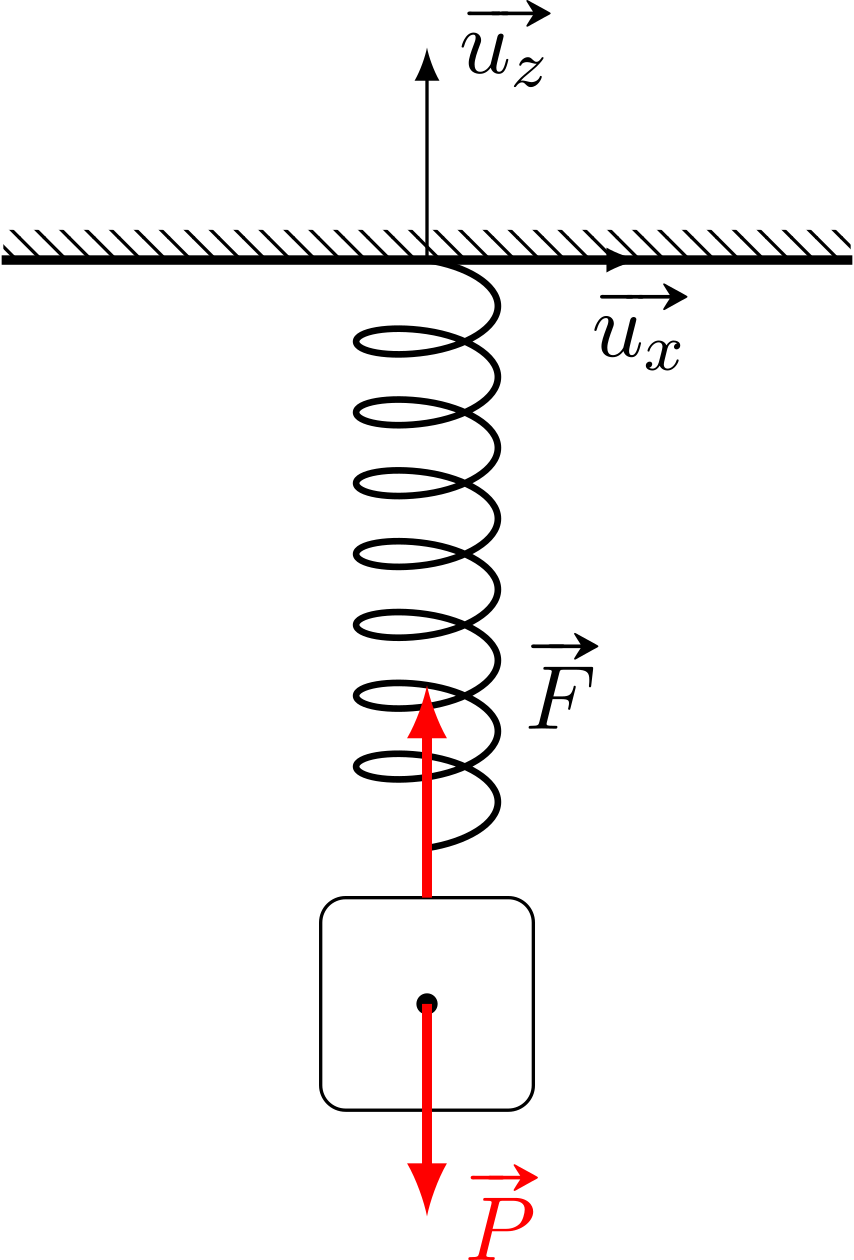
\includegraphics[width=.7\linewidth, draft=true]{ressort_vert}
			}{
				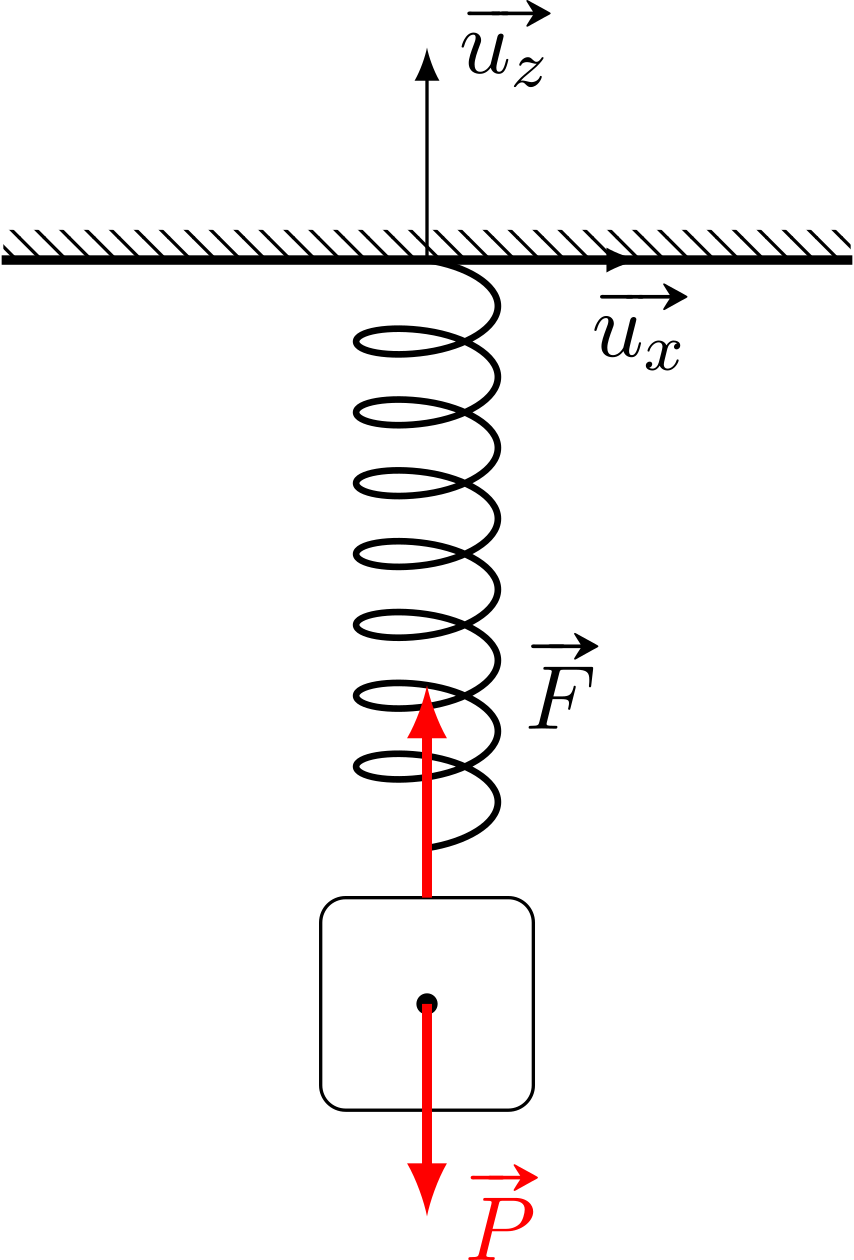
\includegraphics[width=.7\linewidth]{ressort_vert}
			}
			\captionof{figure}{}
		\end{center}
	\end{minipage}
	\vspace{-90pt}
	\psw{
		\begin{enumerate}[label=\sqenumi, start=4]
			\bitem{BdF}~:
			\vspace{-15pt}
			\[
				\begin{array}{ll}
					\pt{1}\textbf{Poids}                & \Pf = m\gf = -mg\uz       \\
					\pt{1}\textbf{Force \textsc{Hooke}} & \Ff = k(\ell - \ell_0)\uz
				\end{array}
			\]
			\bitem{PFD à l'équilibre}~:
			\vspace{-22pt}
			\begin{gather*}
				\of \stm[-1]{=} \sum \Ff\ind{\ext}
				\Lra
				0 = -mg + k(\ell_{\equ} - \ell_0)
				\\\Lra
				k(\ell_{\equ} - \ell_0) = mg
				\Lra
				\boxed{\ell_{\equ} \stm[-1]{=} \ell_0 + \frac{mg}{k}}
			\end{gather*}
		\end{enumerate}
	}
	\nitem{7}%
	Représenter sur un schéma les coordonnées cylindriques. Détaillez les
	projections de $\ur$ et $\ut$ sur la base cartésienne, donner l'expression de
	$\OM$ et $\dd{\OM}$ \xul{sans démonstration}, et démontrer les expressions de
	$\vf$ et $\af$ \textbf{sans démontrer les expressions de $\dv{\ur}{t}$ et
		$\dv{\ut}{t}$}.
	\smallbreak
	\noindent
	\begin{minipage}[t]{.70\linewidth}
		\psw{
			\begin{gather*}
				\beforetext{\pt{1}}
				\ur = \cos(\tt)\ux + \sin(\tt)\uy
				\qet
				\ur = -\sin(\tt)\ux + \cos(\tt)\uy
				\\
				\beforetext{\pt{1}}
				\OM = r\ur + z \uz
				\\
				\beforetext{\pt{1}}
				\dd{\OM} = \dd{r}\ur + r \dd{\tt}\ut + \dd{z}\uz
				\\
				\beforetext{\pt{1}}
				\vf = \dv{\OM}{t} = \rp\ur + r \tp \ut + \zp\uz
				\\
				\af =
				\dv{\tikzmark{DV}}{t}
				\left(
				\rp\tikzmark{RP}\ur\tikzmark{UR} +
				r\tikzmark{R}\tp\tikzmark{TP}\ut\tikzmark{UT} +
				\zp\tikzmark{ZP}\uz
				\right)
				\Lra
				\af \stm{=}
				\lsw{orchid}{\rpp}\ur +
				\rp \lsw{cornflowerblue}{\dv{\ur}{t}} +
				\lsw{limegreen}{\rp}\tp\ut +
				r\lsw{orange}{\tpp}\ut +
				r\tp \lsw{firebrick}{\dv{\ut}{t}} +
				\zpp\uz
				\\\Lra
				\boxed{
					\af \stm[-1]{=} \left( \rpp -r\tp^2 \right)\ur +
					\left( 2\rp\tp + r\tpp \right)\ut +
					\zpp\uz
				}
			\end{gather*}
			\tikz[remember picture, overlay]
			\draw[-stealth, transform canvas={yshift=6pt}, color=\sswitch{white}{orchid}]
			(pic cs:DV) to [out=90, in=90] ([shift={(-3pt,3pt)}]pic cs:RP)
			;
			\tikz[remember picture, overlay]
			\draw[-stealth, transform canvas={yshift=6pt}, color=\sswitch{white}{cornflowerblue}]
			(pic cs:DV) to [out=90, in=90] ([shift={(-6pt,6pt)}]pic cs:UR)
			;
			\tikz[remember picture, overlay]
			\draw[-stealth, transform canvas={yshift=6pt}, color=\sswitch{white}{limegreen}]
			(pic cs:DV) to [out=90, in=90] ([shift={(-3pt,3pt)}]pic cs:R)
			;
			\tikz[remember picture, overlay]
			\draw[-stealth, transform canvas={yshift=6pt}, color=\sswitch{white}{orange}]
			(pic cs:DV) to [out=90, in=90] ([shift={(-3pt,6pt)}]pic cs:TP)
			;
			\tikz[remember picture, overlay]
			\draw[-stealth, transform canvas={yshift=6pt}, color=\sswitch{white}{firebrick}]
			(pic cs:DV) to [out=90, in=90] ([shift={(-6pt,6pt)}]pic cs:UT)
			;
			\tikz[remember picture, overlay]
			\draw[-stealth, transform canvas={yshift=6pt}, color=\sswitch{white}{black}]
			(pic cs:DV) to [out=90, in=90] ([shift={(-3pt,3pt)}]pic cs:ZP)
			;
		}
	\end{minipage}
	\hfill
	\begin{minipage}[t]{.20\linewidth}
		\vspace*{0pt}
		\begin{center}
			\sswitch{
				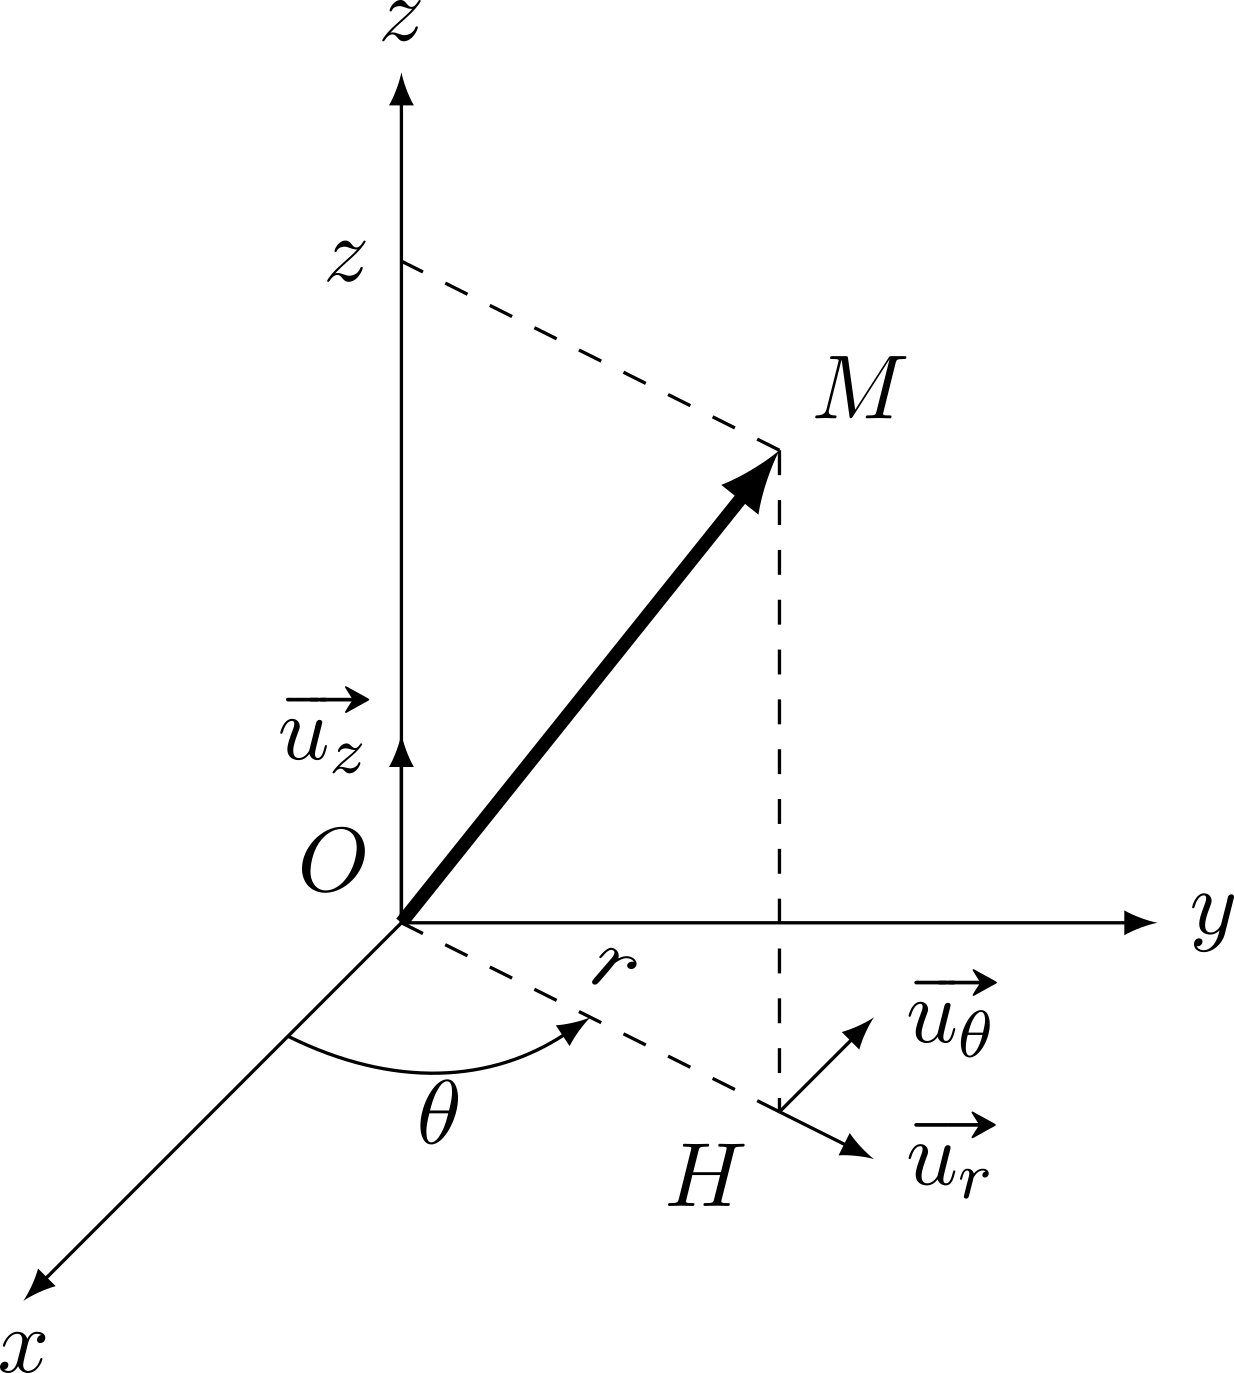
\includegraphics[width=\linewidth, draft=true]{cyl_rep}
			}{
				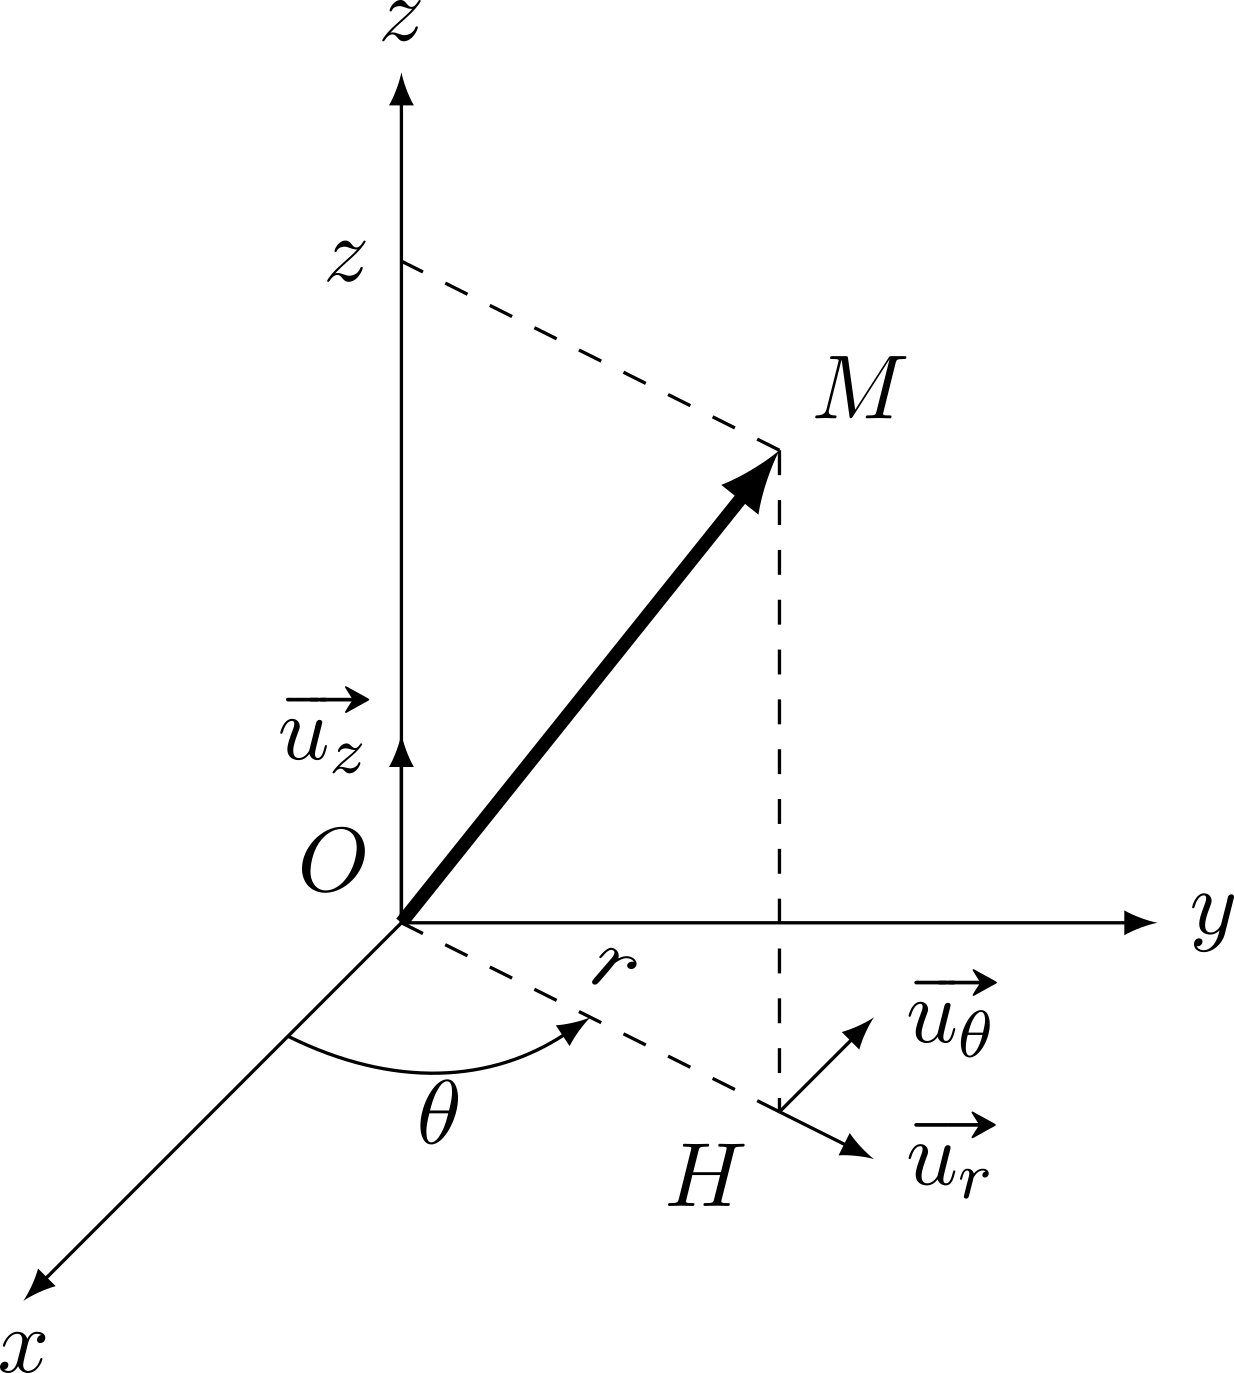
\includegraphics[width=\linewidth]{cyl_rep}
			}
			\vspace{-15pt}
			\captionsetup{justification=centering}
			\captionof{figure}{\smallbreak Cylindriques\protect\pt{1}}
		\end{center}
	\end{minipage}
	\nitem{4}%
	\noindent
	\begin{minipage}[t]{.70\linewidth}
		Projetez $\Pf$ et $\Tf$ dans les conditions de la Figure~\ref{fig:pendule}.
		Avec $\OM = \ell\ur$ et $\lp = 0 = \lpp$ et votre réponse à la question
		précédente, appliquer le PFD pour obtenir deux équations différentielles. Sous
		quelles conditions l'une d'entre elle est celle d'un oscillateur harmonique~?
		\smallbreak
		\psw{
			\begin{gather*}
				\pt{1}
				\begin{array}{ll}
					\textbf{Poids}   & \Pf = m\gf = mg(\cos\tt \ur - \sin\tt \ut)
					\\
					\textbf{Tension} & \Tf = -T\ur
				\end{array}
				\\
				\beforetext{Or,}
				m\af \stm[-1]{=} m (-\ell\tp^2 \ur + \ell\tpp \ut) = \Pf + \Tf
			\end{gather*}
			\begin{empheq}[box=\fbox, left=\stm{\Lra}\empheqlbrace]{align}
				mg\cos\tt + m \ell\tp^2 & = T\notag\\
				\label{eq:pendb}
				m \ell\tpp + mg\sin\tt & = 0
			\end{empheq}
			L'équation~(15.1) est l'équation d'un oscillateur harmonique pour
			des petits angles ($\sin(\theta) \Sim_{\tt\to0} \tt$)\pt{1}.
		}
	\end{minipage}
	\hfill
	\begin{minipage}[t]{0.25\linewidth}
		\vspace*{0pt}
		\begin{center}
			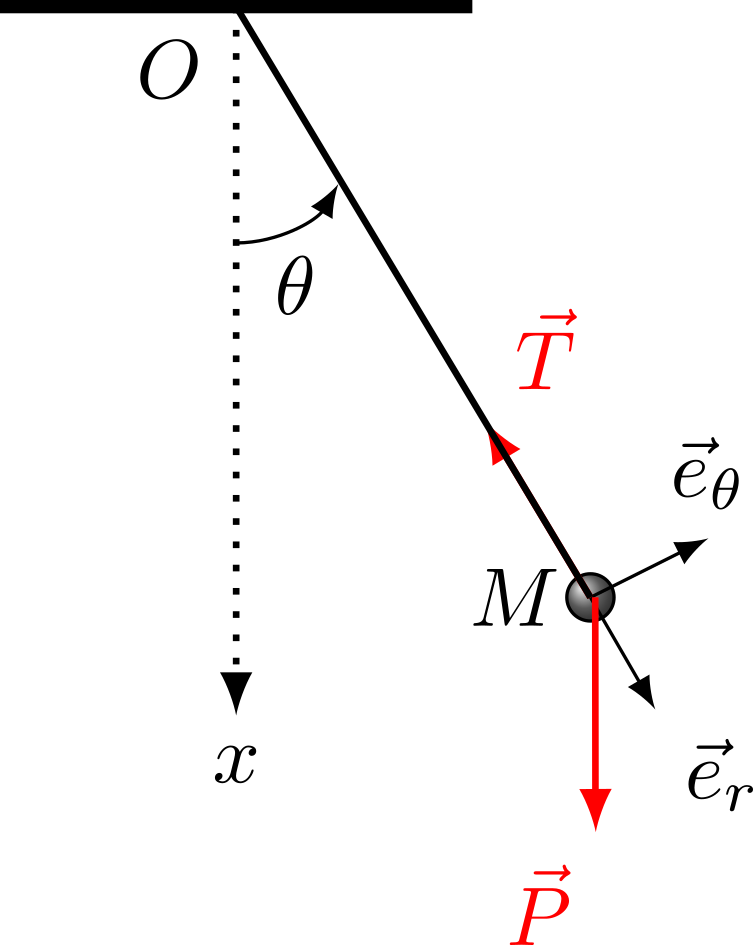
\includegraphics[width=\linewidth]{pendule_plain}
			\captionof{figure}{Schéma}
			\label{fig:pendule}
		\end{center}
	\end{minipage}
	\ifstudent{
		\begin{tikzpicture}[remember picture, overlay]
			\node[anchor=north west, align=left]
			at ([shift={(1.4cm,0)}]current page.north west)
			{\\[5pt]\Large\bfseries Nom~:\\[10pt]\Large\bfseries Prénom~:};
			\node[anchor=north east, align=right]
			at ([shift={(-1.5cm,-17pt)}]current page.north east)
			{\Large\bfseries Note~:\hspace{1cm}/20};
		\end{tikzpicture}
	}
\end{enumerate}
\end{document}
